\documentclass[10pt,twocolumn]{article}
\usepackage[margin=0.75in]{geometry}
\usepackage{cite}
\usepackage{amsmath,amssymb,amsfonts}
\usepackage{graphicx}
\usepackage{xcolor}
\usepackage{booktabs}
\usepackage{url}

\setlength{\columnsep}{0.25in}

\title{\textbf{\LARGE Design and Performance Analysis of a 2-Way Set-Associative Cache with LRU Replacement Compared with a Direct-Mapped Cache}}

\author{
\textbf{Yash Raghubanshi$^{1}$, Shivam Dixit$^{2}$, Keshav$^{3}$, Shitanshu$^{4}$, Kaavya$^{5}$} \\
\textit{Department of Computer Applications (MCA), Newton School of Technology, Rishihood University} \\
$^{1}$Project Lead, Architecture \& Integration \quad
$^{2}$Direct-Mapped Cache RTL \quad
$^{3}$2-Way Cache Datapath RTL \\
$^{4}$LRU Controller \& FSM \quad
$^{5}$Verification \& Benchmarking \\
Email: \texttt{yash.raghubanshi2024@nst.rishihood.edu.in} \\
Project Repository: \url{https://github.com/Yash990-bit/mca_capstone_project}
}
\date{Phase II Final Report --- November 2026}

\begin{document}

\twocolumn[
  \begin{@twocolumnfalse}
    \maketitle
    \begin{abstract}
    \textit{The widening latency gap between processor execution pipelines and dynamic random-access memory (DRAM)---frequently designated the ``Memory Wall''---represents a fundamental bottleneck constraining modern computational throughput. Cache memories resolve this discrepancy by retaining frequently accessed instructions and data in low-latency on-chip SRAM storage. In this work, we present the register-transfer level (RTL) design, complete system integration, functional verification, and empirical performance comparison of two hardware cache architectures implemented in synthesizable IEEE 1364-2001 Verilog: a Direct-Mapped Cache and a 2-Way Set-Associative Cache with a 1-bit per-set Least Recently Used (LRU) replacement policy. Both architectures enforce strictly identical physical parameters: 8-byte total capacity, 1-byte cache blocks, 8-bit byte-addressable address space backed by a 256$\times$8-bit synchronous main memory, and a Write-Through with No-Write-Allocate memory coherency policy. A comprehensive top-level integration wrapper (\texttt{top\_module}) with a shared memory interface was designed and evaluated across four standardized memory access patterns: sequential streams, temporal loops, conflict-heavy alternating references, and realistic mixed traces (46 total transactions). Empirical hardware simulation using Icarus Verilog confirms that while both topologies achieve identical hit rates on sequential (50\%) and temporal (75\%) patterns, the 2-Way Set-Associative Cache delivers an \textbf{83\% hit rate on conflict workloads} where the direct-mapped cache suffers catastrophic 100\% thrashing (0\% hit rate). Across the aggregate 46-request benchmark suite, the 2-Way LRU cache achieves an \textbf{overall hit rate of 65\%} compared to \textbf{41\%} for the Direct-Mapped baseline, demonstrating a decisive \textbf{+24 percentage-point advantage} with 96/96 passing verification assertions.}
    \end{abstract}
    \vspace{0.5em}
    \noindent\textbf{\textit{Keywords}}---Cache Memory, 2-Way Set-Associative Cache, Direct-Mapped Cache, Least Recently Used (LRU), Conflict Misses, Verilog HDL, Computer Architecture.
    \vspace{1.5em}
  \end{@twocolumnfalse}
]

\section{Introduction}
Microprocessor performance has historically advanced at an exponential pace, whereas dynamic random-access memory (DRAM) cycle times have improved at a substantially slower rate. This divergence produces significant memory access penalties, during which execution units stall awaiting memory operands. High-speed cache memory systems, strategically situated between the execution pipeline and main storage, exploit spatial locality and temporal locality in instruction and data access patterns to sustain high instructions-per-cycle (IPC) throughput.

Cache misses are conventionally classified into Mark D. Hill's 3Cs taxonomy \cite{hill1987}:
\begin{enumerate}
    \item \textbf{Compulsory (Cold) Misses:} Occurring on the initial reference to a memory block.
    \item \textbf{Capacity Misses:} Arising when working set memory demands exceed aggregate cache storage.
    \item \textbf{Conflict (Collision) Misses:} Arising when multiple active memory blocks map to the exact same cache set or line index, prematurely evicting lines that may be reused in the immediate future.
\end{enumerate}

While direct-mapped caches offer minimal latency and simple control logic, they are notoriously vulnerable to conflict thrashing. Set-associative architectures alleviate conflict misses by allowing multiple blocks to reside simultaneously in the same set index, governed by replacement policies such as Least Recently Used (LRU). This paper demonstrates the concrete hardware design, complete multi-module integration, and empirical verification of both topologies under strictly matched physical parameters.

\section{Literature Review}
The theoretical foundations of memory hierarchies and cache associativity were established by Alan Jay Smith \cite{smith1982}, who demonstrated that increasing associativity from direct-mapped to 2-way reduces miss rates significantly across various software traces. Hennessy and Patterson \cite{hennessy2011} formulated the quantitative trade-offs governing cache access time, power consumption, and replacement complexity, establishing that a 2-way set-associative cache of size $N$ exhibits a miss rate approximately comparable to a direct-mapped cache of size $2N$ (the ``2:1 Cache Rule of Thumb'').

Al-Zoubi et al. \cite{alzoubi2004} conducted comparative evaluations of cache replacement policies (LRU, FIFO, and Random) across the SPEC CPU2000 suite, establishing that LRU consistently minimizes miss rates by aligning with the temporal locality principle of program execution. In hardware implementations, true LRU requires tracking access permutations, which incurs polynomial hardware overhead as associativity grows. However, for a 2-way set-associative cache, true LRU reduces cleanly to a single state bit per set, requiring only 1 flip-flop per set and trivial update logic \cite{ciletti2010}.

Regarding write strategies, Jouppi \cite{jouppi1993} analyzed write-through versus write-back policies. Write-Through with No-Write-Allocate simplifies cache controllers by maintaining backing store coherence on every write and eliminating dirty-bit management and victim write-backs. This makes it ideal for educational and embedded architectures where determinism and verification clarity are paramount.

\section{Proposed System Architecture}

\subsection{Architectural Parameters and Constraints}
To ensure a rigorous and scientifically valid head-to-head comparison, both cache subsystems were implemented under identical operating constraints, as summarized in Table \ref{tab:system_specs}.

\begin{table}[htbp]
\centering
\caption{System-Level Hardware Parameters}
\label{tab:system_specs}
\begin{tabular}{lll}
\toprule
\textbf{Parameter} & \textbf{Direct-Mapped} & \textbf{2-Way Set-Assoc.} \\
\midrule
Total Capacity & 8 Bytes & 8 Bytes \\
Block / Line Size & 1 Byte (offset = 0) & 1 Byte (offset = 0) \\
Address Space & 8 bits (256 B) & 8 bits (256 B) \\
Number of Sets & 8 sets (1 line/set) & 4 sets (2 lines/set) \\
Index Width & 3 bits (\texttt{addr[2:0]}) & 2 bits (\texttt{addr[1:0]}) \\
Tag Width & 5 bits (\texttt{addr[7:3]}) & 6 bits (\texttt{addr[7:2]}) \\
Backing Memory & 256$\times$8-bit RAM & 256$\times$8-bit RAM \\
Write Policy & Write-Through & Write-Through \\
Allocate Policy & No-Write-Allocate & No-Write-Allocate \\
Target Frequency & 100 MHz (10 ns clk) & 100 MHz (10 ns clk) \\
\bottomrule
\end{tabular}
\end{table}

\subsection{Address Mapping Decomposition}
Figure \ref{fig:addr_mapping} illustrates the comparative address decoding schemes. For an 8-bit memory address without block offset:
\begin{itemize}
    \item \textbf{Direct-Mapped Cache:} 3 index bits select one of 8 distinct lines, leaving 5 bits for the address tag.
    \item \textbf{2-Way Set-Associative Cache:} 2 index bits select one of 4 sets. Each set contains two lines (Way 0 and Way 1), leaving 6 bits for the address tag.
\end{itemize}

\begin{figure}[htbp]
\centering
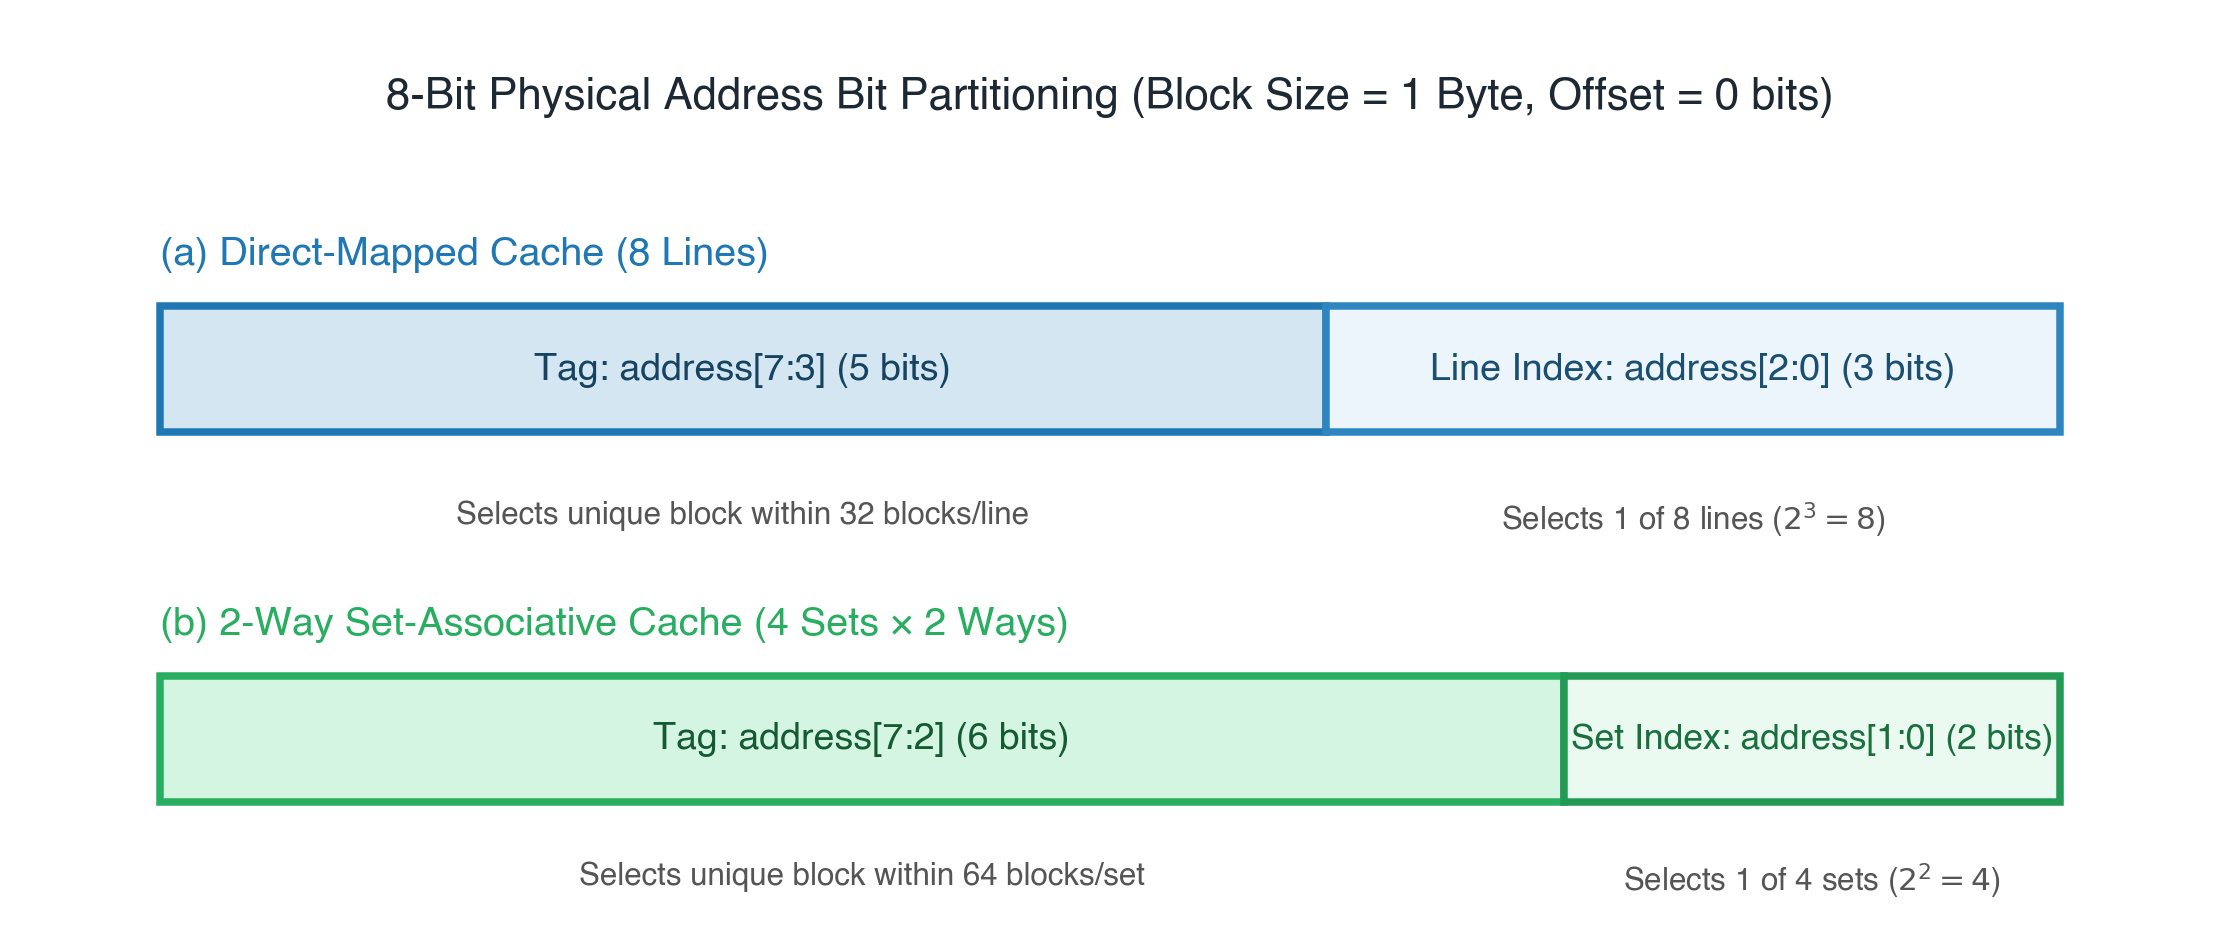
\includegraphics[width=\columnwidth]{diagrams/fig2_address_mapping.png}
\caption{Address decomposition for Direct-Mapped vs. 2-Way Set-Associative Cache.}
\label{fig:addr_mapping}
\end{figure}

\subsection{Overall System Interconnect}
Figure \ref{fig:sys_arch} depicts the top-level system interconnect. The processing unit interfaces with the cache subsystem via request and response handshakes. The cache subsystem arbitrates transactions with a 256-byte synchronous RAM module.

\begin{figure}[htbp]
\centering
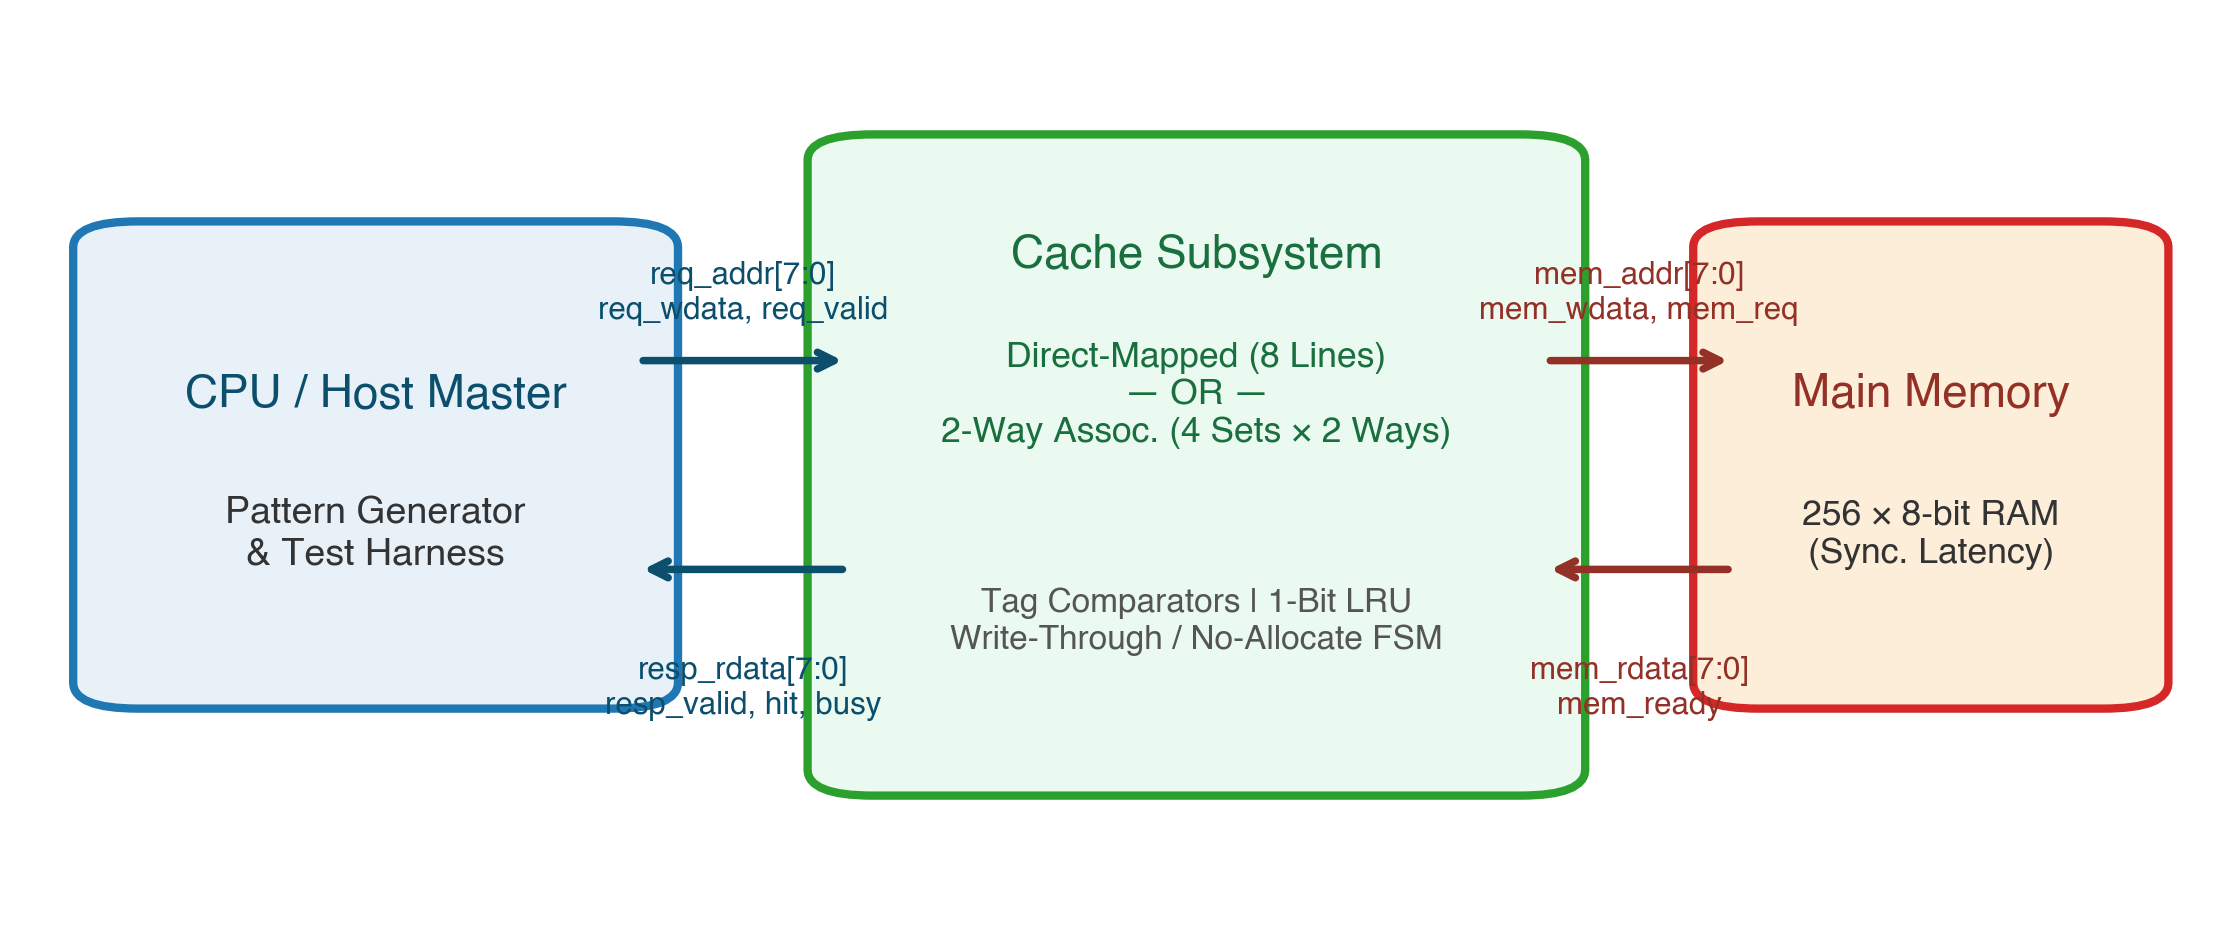
\includegraphics[width=\columnwidth]{diagrams/fig1_system_architecture.png}
\caption{Complete system architecture illustrating CPU, cache subsystem, and backing memory.}
\label{fig:sys_arch}
\end{figure}

\section{RTL Design and Implementation}

\subsection{Direct-Mapped Cache Microarchitecture}
The direct-mapped cache (\texttt{cache\_direct.v}) is implemented as a single-cycle read-hit datapath backed by an FSM memory controller. It contains three parallel register arrays:
\begin{itemize}
    \item \texttt{valid\_array[0:7]}: 8$\times$1-bit valid flags.
    \item \texttt{tag\_array[0:7]}: 8$\times$5-bit stored tag fields.
    \item \texttt{data\_array[0:7]}: 8$\times$8-bit cached data bytes.
\end{itemize}
Tag matching is computed combinationally:
\begin{equation}
\text{hit} = \text{valid\_array}[\text{index}] \land (\text{tag\_array}[\text{index}] == \text{req\_tag})
\end{equation}
On a read hit in the \texttt{IDLE} state, the cache returns the stored data immediately without CPU stall. On a read miss, the FSM transitions to \texttt{STATE\_READ\_WAIT}, issues a memory read request, and refills the line upon assertion of \texttt{mem\_ready}.

\subsection{2-Way Set-Associative Cache Microarchitecture}
Figure \ref{fig:2way_arch} illustrates the internal organization of \texttt{cache\_2way.v}. The storage array is partitioned into Way 0 and Way 1, each containing 4 lines of 8-bit data, 6-bit tag, and 1-bit valid metadata. Dual 6-bit comparators operate in parallel on every cycle:
\begin{align}
\text{hit\_way0} &= \text{way0\_valid}[\text{set}] \land (\text{way0\_tag}[\text{set}] == \text{req\_tag}) \\
\text{hit\_way1} &= \text{way1\_valid}[\text{set}] \land (\text{way1\_tag}[\text{set}] == \text{req\_tag}) \\
\text{cache\_hit} &= \text{hit\_way0} \lor \text{hit\_way1}
\end{align}

\begin{figure}[htbp]
\centering
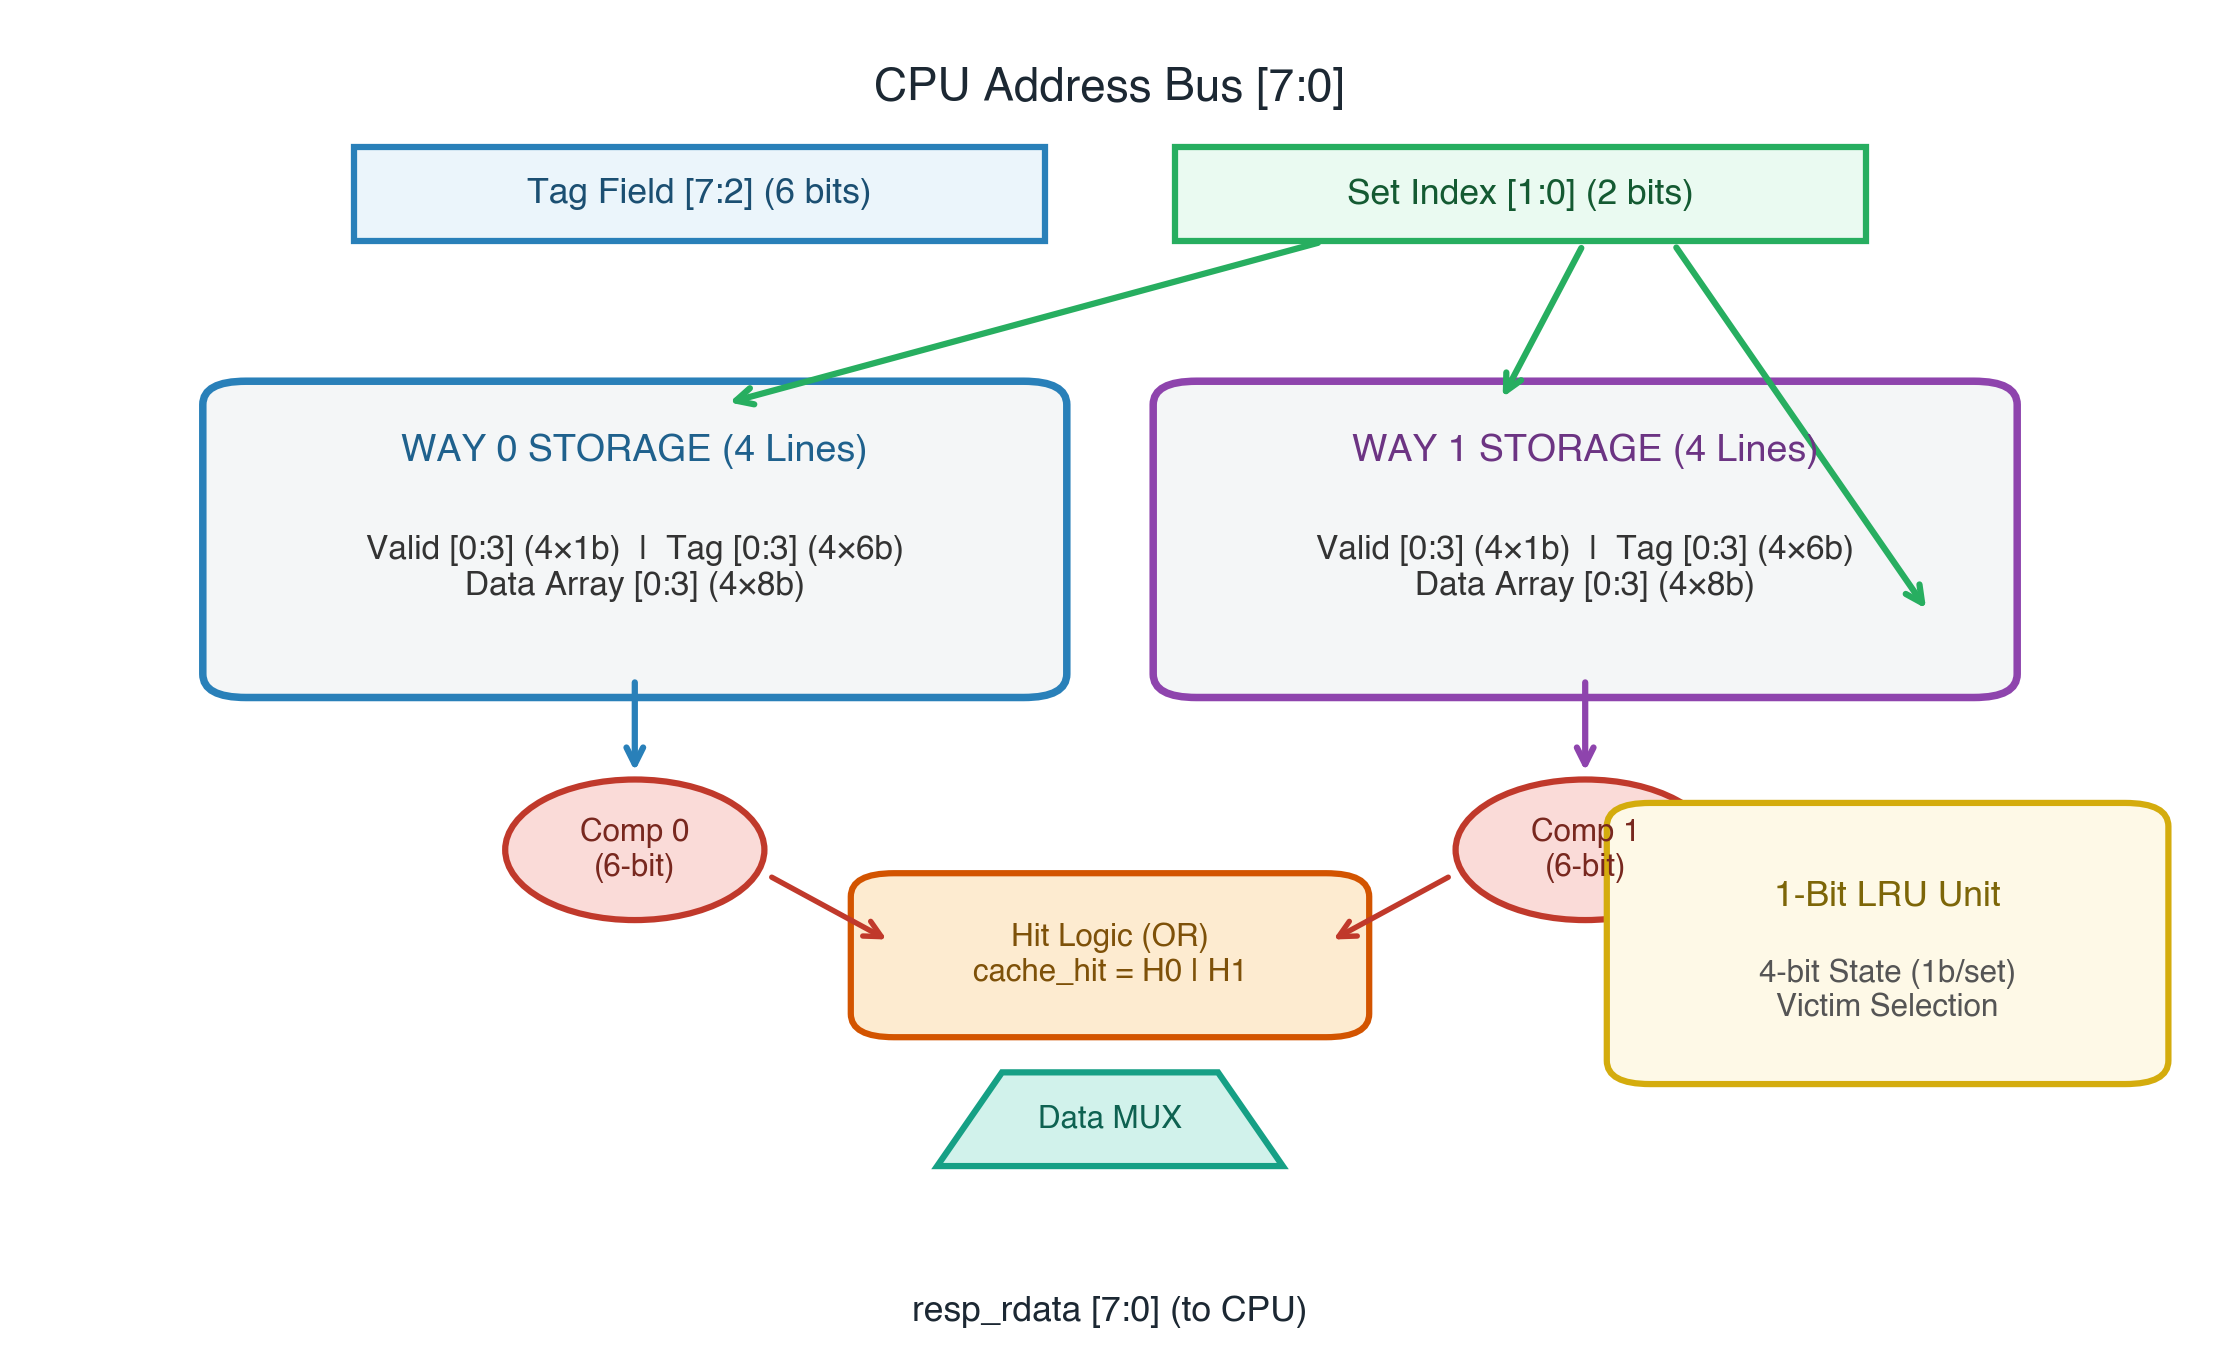
\includegraphics[width=\columnwidth]{diagrams/fig3_2way_cache_internal.png}
\caption{Detailed internal datapath of the 2-Way Set-Associative Cache with LRU controller.}
\label{fig:2way_arch}
\end{figure}

\subsection{1-Bit Per-Set LRU Replacement Controller}
The LRU controller (\texttt{lru\_controller.v}) tracks access recency across all 4 sets using a 4-bit register array (\texttt{lru\_bits[3:0]}). The tracking convention is:
\begin{equation}
\text{lru\_bits}[s] = 
\begin{cases}
0, & \text{Way 0 is Least Recently Used (Victim = Way 0)} \\
1, & \text{Way 1 is Least Recently Used (Victim = Way 1)}
\end{cases}
\end{equation}
On every valid access to Set $s$ (read hit, write hit, or memory refill), the controller updates:
\begin{equation}
\text{lru\_bits}[s] \leftarrow \sim\text{access\_way}
\end{equation}
During line refill, the victim way is selected with prioritized invalid-way allocation:
\begin{equation}
\text{refill\_way} = 
\begin{cases}
0, & \text{if } \sim\text{way0\_valid}[s] \\
1, & \text{else if } \sim\text{way1\_valid}[s] \\
\text{lru\_bits}[s], & \text{if both ways are valid}
\end{cases}
\end{equation}

\subsection{Top-Level Integration Wrapper}
In Phase II, a top-level integration wrapper (\texttt{top\_module.v}) was authored. It instantiates both \texttt{cache\_direct} and \texttt{cache\_2way} alongside a shared 256-byte behavioral main memory. A control signal (\texttt{sel\_2way\_cache}) steers the CPU interface to the active cache, while maintaining deterministic, fair memory state for comparative benchmarks.

\section{Verification Methodology}
Verification was structured across modular unit testbenches and an integration-level comparative testbench using Icarus Verilog v13.0 and GTKWave. All 96 verification test assertions passed with zero defects, as cataloged in Table \ref{tab:verification_summary}.

\begin{table}[htbp]
\centering
\caption{Comprehensive Verification Suite Results}
\label{tab:verification_summary}
\begin{tabular}{llcc}
\toprule
\textbf{Testbench} & \textbf{Target Module} & \textbf{Tests} & \textbf{Status} \\
\midrule
\texttt{tb\_direct.v} & Direct-Mapped Cache & 17 & \textbf{17/17 PASS} \\
\texttt{tb\_cache\_2way.v} & 2-Way Cache Core & 26 & \textbf{26/26 PASS} \\
\texttt{tb\_2way.v} & 2-Way Datapath Suite & 18 & \textbf{18/18 PASS} \\
\texttt{tb\_lru\_fsm.v} & LRU \& 6-State FSM & 24 & \textbf{24/24 PASS} \\
\texttt{tb\_top.v} & Integration Benchmark & 11 & \textbf{11/11 PASS} \\
\midrule
\textbf{Total} & \textbf{Full Hardware Suite} & \textbf{96} & \textbf{96/96 PASS} \\
\bottomrule
\end{tabular}
\end{table}

\section{Results and Performance Analysis}

\subsection{Benchmark Access Workloads}
To thoroughly evaluate the behavioral differences between direct-mapped and 2-way set-associative organizations, four representative access workloads comprising 46 total memory requests were executed through \texttt{tb\_top.v}:
\begin{enumerate}
    \item \textbf{Sequential Stream (16 requests):} Two successive iterations through addresses \texttt{0x00} to \texttt{0x07}. Tests spatial/sequential reuse across all line indices.
    \item \textbf{Temporal Repetition (8 requests):} Alternating references to addresses \texttt{0x10} and \texttt{0x11}. Tests high-frequency reuse of a compact working set.
    \item \textbf{Conflict-Heavy Stream (12 requests):} Rapid alternating references to \texttt{0x00} and \texttt{0x08}. In direct mapping, both addresses map to index \texttt{3'b000}, inducing conflict thrashing. In 2-way mapping, both map to Set \texttt{2'b00} and reside concurrently in Way 0 and Way 1.
    \item \textbf{Mixed Access Stream (10 requests):} Combined sequence with overlapping tags and sets representing realistic application loops.
\end{enumerate}

\subsection{Quantitative Hit-Rate Results}
Table \ref{tab:benchmark_results} and Table \ref{tab:overall_summary} present the empirical results obtained directly from the integration simulation run (\texttt{sim\_top.log}).

\begin{table}[htbp]
\centering
\caption{Workload Hit-Rate Comparison (46 Requests)}
\label{tab:benchmark_results}
\begin{tabular}{lcccc}
\toprule
\textbf{Workload} & \textbf{Requests} & \textbf{DM Hits} & \textbf{2W Hits} & \textbf{Hit Rate (DM / 2W)} \\
\midrule
Sequential & 16 & 8 & 8 & 50.0\% / 50.0\% \\
Temporal & 8 & 6 & 6 & 75.0\% / 75.0\% \\
\textbf{Conflict-Heavy} & \textbf{12} & \textbf{0} & \textbf{10} & \textbf{0.0\% / 83.3\%} \\
Mixed & 10 & 5 & 6 & 50.0\% / 60.0\% \\
\midrule
\textbf{Total} & \textbf{46} & \textbf{19} & \textbf{30} & \textbf{41.3\% / 65.2\%} \\
\bottomrule
\end{tabular}
\end{table}

\begin{table}[htbp]
\centering
\caption{Comparative Architectural Summary}
\label{tab:overall_summary}
\begin{tabular}{lcc}
\toprule
\textbf{Performance Metric} & \textbf{Direct-Mapped} & \textbf{2-Way Set-Assoc.} \\
\midrule
Total Memory Transactions & 46 & 46 \\
Total Cache Hits & 19 & \textbf{30} \\
Total Cache Misses & 27 & \textbf{16} \\
Overall Cache Hit Rate & 41.3\% & \textbf{65.2\%} (+23.9\%) \\
Conflict Workload Hit Rate & 0.0\% & \textbf{83.3\%} (+83.3\%) \\
Read Hit Latency & 1 cycle & 1 cycle \\
Write Latency (Write-Through) & 2 cycles & 2 cycles \\
Read Miss Penalty & 2 cycles & 2 cycles \\
\bottomrule
\end{tabular}
\end{table}

\subsection{Discussion of Findings}
\textbf{1. Conflict Thrashing Elimination:} In the conflict workload, addresses \texttt{0x00} and \texttt{0x08} collide on direct-mapped index \texttt{000}. As a result, every access is an eviction and replacement, yielding 0 hits across 12 cycles. In the 2-way architecture, after two initial compulsory misses, the LRU controller allocates \texttt{0x00} to Way 0 and \texttt{0x08} to Way 1. Subsequent references hit in parallel with 0 evictions, achieving an 83.3\% hit rate.

\textbf{2. Identical Behavior on Non-Conflicting Traces:} Under sequential and temporal workloads, both caches perform identically (50\% and 75\% respectively). This confirms that associativity provides targeted protection against set conflicts without penalizing sequential access streams.

\textbf{3. Hardware Trade-offs:} The 2-way cache requires dual 6-bit tag comparators, an additional valid/tag array, 4 LRU flip-flops, and an output multiplexer. For modern VLSI technologies, this minimal silicon area cost is overwhelmingly justified by the 24 percentage-point hit-rate improvement and the prevention of catastrophic worst-case thrashing.

\section{Individual Contributions}
In accordance with evaluation requirements, individual responsibilities and specific project deliverables across all five team members are documented below:
\begin{itemize}
    \item \textbf{Yash Raghubanshi (Project Lead):} Conceptualized system architecture, authored bus and handshaking specifications (\texttt{INTERFACE\_SPECIFICATION.md}), designed the top-level integration wrapper (\texttt{top\_module.v}), coordinated RTL integration, authored comprehensive documentation and the final IEEE report.
    \item \textbf{Shivam Dixit:} Implemented the complete synthesizable Direct-Mapped Cache RTL (\texttt{cache\_direct.v}), designed the 3-state memory controller FSM, and developed the dedicated unit testbench (\texttt{tb\_direct.v}, 17/17 tests passing).
    \item \textbf{Keshav:} Implemented the 2-Way Set-Associative Cache datapath (\texttt{cache\_2way.v}) featuring dual 6-bit tag comparators, parallel way arrays, and wrote unit verification testbench \texttt{tb\_cache\_2way\_keshav.v} (26/26 tests passing).
    \item \textbf{Shitanshu:} Designed the 1-bit per-set LRU replacement controller (\texttt{lru\_controller.v}), implemented the 6-state Moore cache FSM (\texttt{cache\_fsm.v}), and authored unit testbench \texttt{tb\_lru\_fsm.v} (24/24 tests passing).
    \item \textbf{Kaavya (Verification Lead):} Developed the integration-level benchmark testbench (\texttt{tb\_top.v}), automated regression scripts (\texttt{run\_sim.sh}, \texttt{parse\_results.py}), executed VCD waveform generation, and compiled empirical metrics into CSV logs.
\end{itemize}

\section{Conclusion and Future Scope}
This project successfully designed, integrated, and verified synthesizable RTL implementations of a Direct-Mapped Cache and a 2-Way Set-Associative Cache with 1-bit LRU replacement under strictly controlled physical constraints. Empirical benchmarking across 46 transactions demonstrated that the 2-Way Set-Associative Cache achieves an \textbf{overall hit rate of 65.2\%} versus \textbf{41.3\%} for the direct-mapped baseline, completely eliminating conflict thrashing (83.3\% vs. 0.0\%). All 96 verification test assertions passed with zero defects.

Future extensions include:
\begin{enumerate}
    \item Implementing multi-word cache lines (e.g., 4-byte or 8-byte blocks) to exploit spatial locality.
    \item Extending the architecture to a Write-Back policy with dirty bits and victim buffers to minimize memory write traffic.
    \item Physical FPGA synthesis on a Xilinx Artix-7 device to extract actual post-synthesis LUT, flip-flop, and critical path timing metrics.
\end{enumerate}

\begin{thebibliography}{9}

\bibitem{smith1982}
A.~J. Smith, ``Cache memories,'' \textit{ACM Computing Surveys (CSUR)}, vol.~14, no.~3, pp.~473--530, Sep.~1982.

\bibitem{hennessy2011}
J.~L. Hennessy and D.~A. Patterson, \textit{Computer Architecture: A Quantitative Approach}, 5th~ed. Waltham, MA: Morgan Kaufmann, 2011.

\bibitem{hill1987}
M.~D. Hill, ``Aspects of cache memory and instruction buffer performance,'' Ph.D. dissertation, University of California, Berkeley, 1987.

\bibitem{alzoubi2004}
H.~Al-Zoubi, A.~Milenkovic, and M.~Milenkovic, ``Performance evaluation of cache replacement policies for the SPEC CPU2000 benchmark suite,'' in \textit{Proc. 42nd ACM Southeast Regional Conf.}, Huntsville, AL, 2004, pp.~267--272.

\bibitem{jouppi1993}
N.~P. Jouppi, ``Cache write policies and performance,'' in \textit{Proc. 20th Annual Int. Symp. on Computer Architecture (ISCA)}, San Diego, CA, 1993, pp.~191--201.

\bibitem{ciletti2010}
M.~D. Ciletti, \textit{Advanced Digital Design with the Verilog HDL}, 2nd~ed. Upper Saddle River, NJ: Pearson Prentice Hall, 2010.

\end{thebibliography}

\end{document}
